\chapter{System description}\label{se:system_description}
This section will go into details of the structure of the sewer network for which the further work of this project will be based upon.

As mentioned in section \ref{se:chemical_process} a steady flow of sewage with a fixed level of contaminants is desired such that an optimal utilization of the wastewater treatment plant can be obtained. An area of interest is Fredericia with a sizable population of around 40.000 and industries where some of the largest consists of a brewery, bottling plant, refinery and a dairy plant \citep{Statistic_Denmark}. All of these industries is placed in the outskirt of the city, meaning that wastewater discharge from any of them into the sewer goes through populated areas creating an uneven flow of sewage to the wastewater treatment plant. Two main sewer lines separates the northern and southern part of the city. To limit the project the northern main sewer line is considered, which covers the largest part of the city and the industry, excluding the dairy from the scope of the project. In figure \ref{fig:kloakgrid_simplified} a simplified overview of the northern main sewer line attached to the various population and industrial areas of Fredericia. The placement of the sewers shown in \ref{fig:kloakgrid_simplified} is obtained from a Geographically Information System (GIS) map \cite{GIS_kort}.     

\begin{figure}[H]
\centering
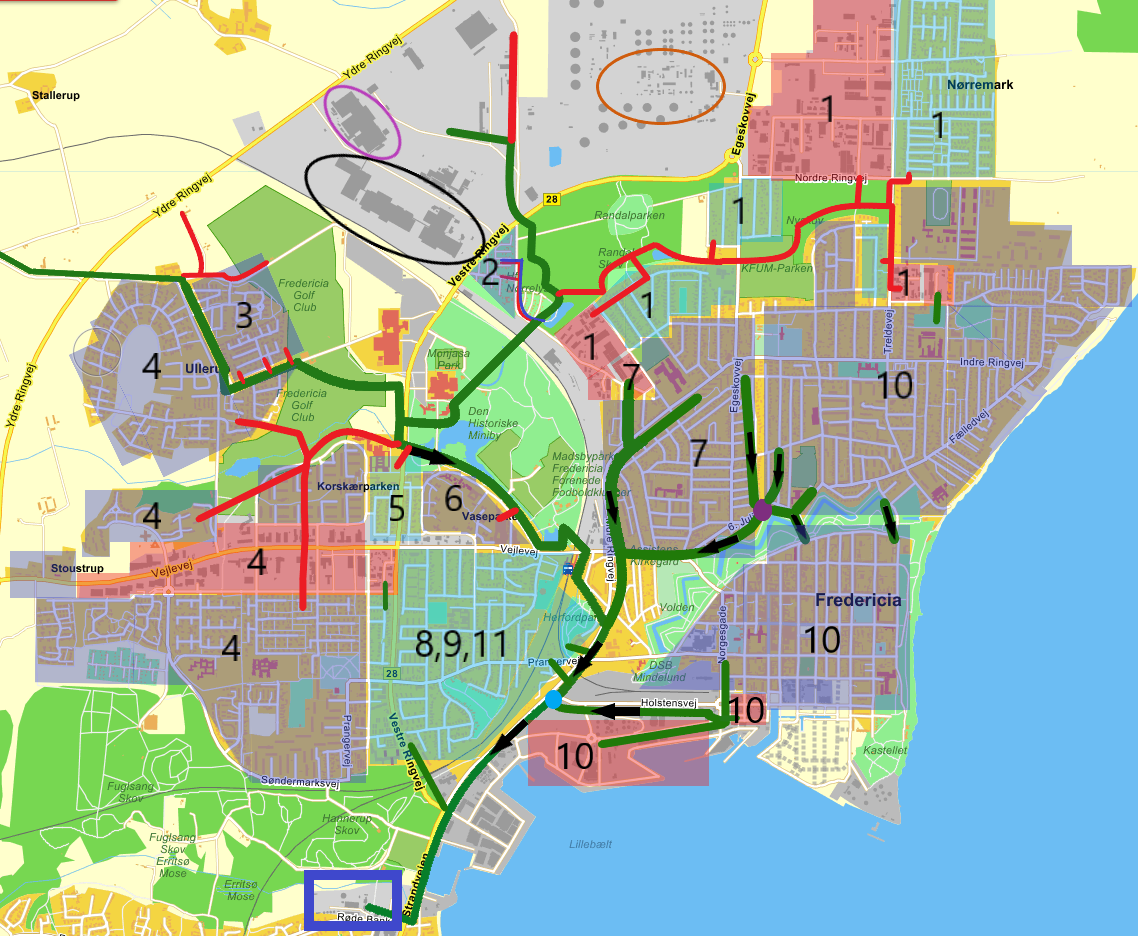
\includegraphics[width=1\textwidth]{report/system_overview/pictures/kloakgrid_simplified8.png}
\caption{Mapping of part of the sewer network in Fredericia. The red and green lines indicate sewers where the red sewers has flows of sewage only and the green line is combined sewage and runoff from urban surfaces. Transparent parts indicate that the area has a connected sewer grid within and the red/green lines from this grid indicates the output from this area. Two shades of transparent blue is used to illustrate sewer systems in populated areas. The red transparent areas indicate minor industry and the black, brown and purple rings is brewery, refinery and bottling plant respectively. The purple dot indicate a connecting point with several incoming and outgoing sewer pipes. The blue dot is a sewer reservoir \fixme{this is a guess pt. so might need to be corrected} before wastewater is led to the wastewater treatment plant indicated by the blue rectangle.}
\label{fig:kloakgrid_simplified}
\end{figure}



\begin{figure}[H]
\centering
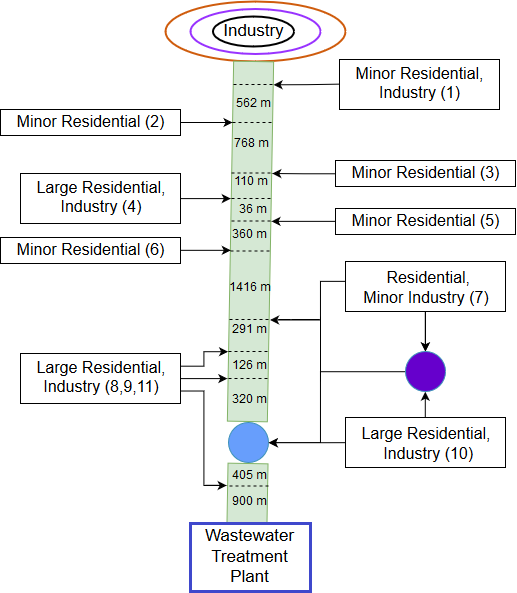
\includegraphics[width=0.8\textwidth]{report/system_overview/pictures/sewer_line_diagram2.png}
\caption{Simplification of the map shown in figure \ref{fig:kloakgrid_simplified} where the numbers correspond to which area is connected to the main sewer line furthest from the wastewater treatment plant and the distance between the connections.}
\label{fig:sewer_line_diagram}
\end{figure}